%% The following is a directive for TeXShop to indicate the main file
%%!TEX root = diss.tex

\chapter{Introduction}
\label{ch:Introduction}

%\begin{epigraph}
%   \emph{If I have seen farther it is by standing on the shoulders of Giants.} ---~Sir Isaac Newton (1855)
%\end{epigraph}

%This first paragraph will give a little intro and describe what is coming up in \autoref{sec:Cosmology}, \autoref{sec:Lensing} and \autoref{sec:Clusters}. The \acf{CFHTLenS} was a big lensing project in the \acf{CFHTLS} survey. This is an example of an acronym that does not go in the table of acronyms:  \acs{UBC}. 

This thesis is concerned with weak gravitational lensing studies of galaxy clusters, using two complementary approaches, shear and magnification. This introductory chapter provides the necessary background and context for understanding the novel research presented in the subsequent chapters. The basics of cosmology, which is the larger field within which this thesis research resides, is given in \autoref{sec:Cosmology}, with a particular focus on distances, which will be important for the presentation of gravitational lensing in \autoref{sec:Lensing}. Galaxy clusters are discussed in \autoref{sec:Clusters}, from the cosmological as well as the intracluster physics perspective. \autoref{sec:Impact} outlines the novelty and importance of the research contained in this thesis. A brief overview of the body of work which is presented in the main chapters of this thesis is given in \autoref{sec:Overview}.

%%%%%%%%%%%%%%%%%%%%%%%%%%%%%%%%%%%%%%%%%%%%%%%%%%%%%%%%%%%%%%%%%%%%%%
\section{Cosmology}
\label{sec:Cosmology}

Cosmology is the study of our universe as a whole. It can be easy to take for granted the simple fact that we, as scientists, can even do cosmology at all -- that is, we can make quantitative and testable predictions about the physical nature of the vast universe we inhabit. At the same time, as we cosmologists forge ahead, caught up in the day-to-day struggles that concern some minute detail of a model, a prediction, or an idea, it is easy to overlook the sheer beauty of what we are so deeply invested in. The introduction of this thesis serves both to lay the requisite theoretical foundation, upon which the thesis research relies, while also giving an honest depiction of the big picture ideas for which this work strives to be relevant.

"The Cosmos is all that is or was or ever will be. Our feeblest contemplations of the Cosmos stir us -- there is a tingling in the spine, a catch in the voice, a faint sensation, as if a distant memory, of falling from a height. We know we are approaching the greatest of mysteries" \citep{Sagan80}.


\subsection{Our Universe}

Looking out into the night sky from our vantage point on planet earth, the universe appears full of structure on many scales. Planets orbiting stars; stars bound into star clusters and galaxies; galaxies themselves organized into clusters ranging from small associations like our local group, to enormous conglomerates of many thousands of galaxies. But if we adopt a holistic mindset on the scale of around 100 Megaparsecs (Mpc), and ignore the smaller scale density fluctuations which are so crucial to our own existence, we observe two remarkable apparent realities of our universe \citep{RydenText}:
\begin{enumerate}
\item {\bf Isotropy.} On large scales, the universe is the same in all locations. There are no special or unique locations.
\item {\bf Homogeneity.} On large scales, the universe is the same in all directions. There are no preferred directions.
\end{enumerate}
These two postulates, which are supported by observations, form the foundation of the current standard cosmological model \citep{BS01}.

A third important fact about our universe on large scales, is that it is expanding. Galaxies are moving away from all other galaxies, at a rate proportional to their distance.\footnote{Note: the linear Hubble relation only holds for relatively small cosmic distances, below a few hundred Mpc \citep{RydenText}.} This simple relationship was discovered by \citet{Hubble29}, and can be expressed as
\begin{equation}
v \approx H_0 r,
\end{equation}
where $v$ is recessional velocity, $r$ is distance, and $H_0$ is known as the Hubble constant \citep{RydenText}. Our current best estimate is $H_0 = 67.8\pm0.77$ km/s/Mpc \citep{PlanckXVI}; this and other cosmological constants are listed in \autoref{table:constants}. The discovery of the expansion of the universe simultaneously abolished any notion that our universe was static, while also giving rise to the idea of a Big Bang origin. Extrapolating back in time, it seems that the universe was once much smaller, denser, and hotter. 

Several pieces of evidence, including the remarkable success of \acf{CMB} experiments such as the \acf{COBE} \citep{COBE96}, the \acf{WMAP} \citep{WMAP9} and \acs{Planck} \citep{PlanckXVI}, provide very strong support for the Big Bang theory. First detected by \citet{PenziasWilson65}, the \ac{CMB} is an isotropic background of microwave photons that have been essentially free-streaming since the universe was a dense opaque cloud. At around 380,000 years of age, the density had dropped sufficiently, and the universe had cooled enough for neutral atoms to form, freeing the photons from constant Thomson scattering. The \ac{CMB} photons match a blackbody spectrum with temperature $2.73 K$ and have a number density of $4.11 \times 10^8 / m^3$. The tiny fluctuations in \ac{CMB} temperature on the sky, which are of order 1 part in $10^5$, are the seeds of structure formation in the universe \citep{RydenText}. Measurements of these anisotropies by \ac{WMAP} and \acs{Planck} have provided cosmological parameter constraints of incredible precision (see \autoref{table:constants}).

One consequence of the expansion of the universe (and also the way it was first discovered) is that light from distant objects is redshifted as it travels to us. This shifts the spectrum of light emitted by galaxies, so that known absorption lines will appear at different wavelengths than they are observed in laboratories on earth. This cosmological redshift can be expressed in terms of the observed and the emitted wavelengths \citep{RydenText}:
\begin{equation}
z \equiv \frac{\lambda_{\rm obs} - \lambda_{\rm em}}{\lambda_{\rm em}}.
\end{equation}

Redshift is often a convenient means of indicating cosmological distances, and will be used frequently throughout this thesis. Since the universe is expanding, it is convenient to express its growth in terms of a scale factor $a(t)$. We define $a$ to be unity today ($a(t_0)=1$), and say that $a(t)<1$ in the past. In this framework we can directly convert the cosmological redshift of an object to the scale factor when its light was emitted \citep{RydenText}:
\begin{equation}
1+z = \frac{a(t_0)}{a(t_{\rm e})} = \frac{1}{a(t_{\rm e})}.
\label{eq:z}
\end{equation}

The expansion history, given by the scale factor $a(t)$, depends upon the constituents of the energy density of the universe. Numerous studies show that, in addition to obvious stuff like normal matter\footnote{Normal matter consists of atoms and other standard model particles, which, in cosmology, are typically all lumped together under the label ``baryonic matter'' despite the fact that they are not all strictly baryons in the particle physics sense \citep{RydenText}.} and radiation, the universe also contains copious amounts of cold dark matter and some form of dark energy, possibly a cosmological constant \citep{DodelsonText}. These components will be discussed in more detail below. This dark sector actually makes up the majority of the present energy density of the universe, but that was not always the case because of the way the density of each component evolves differently with the scale factor.

\subsection{Dark Matter}
\label{sec:DM}

The notion of an invisible dark matter has been around for a surprisingly long time. The idea was first proposed by \citet{Zwicky33} to explain the fact that the mass of the Coma Cluster estimated from radial velocities of member galaxies greatly exceeded the mass estimated from luminosity \citep[see also][]{Zwicky37}. Several years later a similar mismatch was observed between the rotation curves of individual galaxies and the amount of visible matter they contained \citep{Babcock39}, indicating that an enormous amount of invisible mass must extend far beyond the visible range of the galaxies. This gave rise to the concept of the dark matter halo, a much larger spherical halo of invisible dark matter existing around every galaxy and galaxy cluster \citep[see][for a review of dark matter's discovery]{Bergh99}.

Current measurements confirm the existence of dark matter, refining its abundance to around 30\% of the energy content of the entire universe -- an order of magnitude greater average density than ordinary matter. For much of the latter part of the 20th century it was thought that the dark matter could simply be normal matter that was not giving off light. Faint stars, brown dwarfs, black holes, rocky bodies, and an abundance of light weight neutrinos, were all candidates for the non-luminous material \citep{Bergh99}. The now mainstream idea of a non-baryonic cold dark matter was first introduced in 1983 by Bond et al. at the Third Moriond Astrophysics Meeting \citet{Bond83}. Cold dark matter is supported by requirements for structure formation in the universe \citep{BS01}, as well as more ``direct'' evidence of the non-interaction of dark matter studied in several merging galaxy cluster systems, including the well-known Bullet Cluster \citep{Clowe06}.

Dark matter seems to interact only through gravity, and certainly not via the electromagnetic force (it does not emit, absorb, or reflect light). The most plausible contender for the actual dark matter particle is called a \acf{WIMP}, which, as the name implies, is a massive particle that interacts only through gravity and the weak nuclear force. Common supersymmetric extensions to the Standard Model of particle physics include particles that could be candidates for \ac{WIMP}s \citep{DodelsonText}. Unfortunately, direct detection of these particles has proved extremely difficult, despite the fact that numerous groups are pursuing detection using a variety of approaches. One group has claimed a WIMP detection (this is the DAMA/LIBRA experiment which has observed an annual signal modulation), but it remains controversial and seems to be ruled out by other experiments (particularly the XENON-100 experiment) \citep{Snowmass13}.

\subsection{Dark Energy}
\label{sec:DE}

Probably the biggest mystery in all of physics is the nature of dark energy. Like dark matter, the idea has been around for many decades, but unlike dark matter it was not initially based upon observations, but rather a preconceived bias. Since this was before Hubble had discovered the expansion of space, Einstein (and many others) assumed the universe was static. But a matter dominated universe described by Einstein's theory of relativity couldn't be static -- it would contract and fall back on itself due to the gravitational potential of all the mass in it \citep{RydenText}. 

Einstein added a term to his field equations known as the cosmological constant, which was supposed to be a repulsive term that perfectly balanced the universe against gravitational collapse. These equations described how the geometry (left-hand-side) was related to the energy content (right-hand-side) of the universe:
\begin{equation}
R_{\mu\nu} - \frac{1}{2} g_{\mu\nu} R =  -\frac{8\pi G}{c^4} T_{\mu\nu} + \Lambda g_{\mu\nu}
\label{eq:Einstein}
\end{equation}
Here $R_{\mu\nu}$ and $R$ are the Ricci tensor and scalar. $G$ is Newton's gravitational constant and $c$ is the speed of light in a vacuum. The metric tensor is given by $g_{\mu\nu}$,  and the energy-momentum tensor is $T_{\mu\nu}$ \citep{Bertone05}. When the Hubble expansion was discovered, Einstein famously abandoned the cosmological constant term, $\Lambda g_{\mu\nu}$, but it has since reappeared \citep{RydenText}.

In the late 1990s, two teams of astronomers were trying to measure the deceleration of the universe, since the current expansion was expected to be slowing under the gravitational attraction of all the matter. Both the High-$z$ Supernovae Search Team \citep{Riess98} and the Supernovae Cosmology Project \citep{Perlmutter99} used type Ia supernovae as standard candles, relating the peak luminosity to the width of the light-curve, and found evidence for a non-zero cosmological constant. The universe's expansion was actually accelerating. This nobel-prize-winning discovery has been a paradigm shift for the field of cosmology.

The name dark energy refers to the unknown force causing the universe to accelerate. The simplest possibility would be a cosmological constant, perhaps a vacuum energy that is uniform throughout space.\footnote{Unfortunately, calculating the expected energy density of the vacuum from particle physics gives a value 124 orders of magnitude higher than observed. This is a major unsolved issue in theoretical physics and cosmology \citep{RydenText}.} Other more complicated theories have been invented to explain the acceleration, so dark energy is the more general term encompassing them all, but currently the data are consistent with a cosmological constant making up almost 70\% of the energy-density of the universe \citep{PlanckXVI}.

\subsection{Cosmic Dynamics}
\label{sec:Dynamics}

General Relativity stipulates that space and time are part of a single fabric, known as space-time. Events separated in this 4-dimension space-time can be described using the Robertson-Walker metric. This particular form of the metric is a direct consequence of the assumptions of homogeneity and isotropy of the universe \citep{Bertone05}:
\begin{equation}
{\rm d}s^2 = -c^2 {\rm d}t^2 +a(t)^2 \left[{\rm d}r^2 + S_{\rm k}(r)^2{\rm d}\Omega^2\right].
\label{eq:metric}
\end{equation}
Here d$t$ is an interval of proper time, d$\Omega^2 = {\rm d}\theta^2 + {\rm sin}^2\theta {\rm d}\phi^2$, and $(r,\theta,\phi)$ are the set of comoving position coordinates (comoving coordinates grow along with the Hubble expansion -- see \autoref{sec:distances}). 

The $S_{\rm k}(r)$ term is specified by the curvature of the universe, which can be {\it flat} (zero curvature, Euclidean), {\it closed} (positively curved, analogous to the surface of a sphere in 2-dimensions), or {\it open} (negatively curved, like the surface of a saddle in 2-dimensions). Explicitly,
\begin{equation}
S_{\rm k}(r) = 
    \begin{cases}
        {\cal R}{\rm sin}(r/{\cal R}), & \text{for positive curvature} \\
        r,              & \text{for zero curvature} \\
        {\cal R}{\rm sinh}(r/{\cal R}), & \text{for negative curvature.}
    \end{cases}
\end{equation}
If curvature is non-zero, then $\cal R$ gives the radius of curvature \citep{RydenText}. Strong limits have been placed on curvature, and it turns out our universe is flat, or extremely close to flat. The fraction of the energy density of the universe contained in curvature is less than about one part in 1000 and is consistent with zero \citep{PlanckXVI}.

Applying the Robertson-Walker metric (\autoref{eq:metric}) to the Einstein field equations (\autoref{eq:Einstein}), we obtain the Friedmann Equation:
\begin{equation}
\left( \frac{\dot a}{a} \right)^2 = \frac{8\pi G}{3} \rho_{\rm total}.
\end{equation}
Here $a=a(t)$ is the scale factor, and $\dot a$ is its first order derivative with respect to time. The total energy density of the universe $\rho_{\rm total}$ appears to be equal to the critical energy density $\rho_{\rm crit}$, which is exactly the case if the universe has zero curvature. The critical density is given by \citep{RydenText}:
\begin{equation}
\rho_{\rm crit}(z) \equiv \frac{3H(z)^2}{8\pi G},
\end{equation}
and its current value is:
\begin{equation}
\rho_{\rm crit}(0) \approx 9.2 \times 10^{-27} {\rm kg}/{\rm m}^{3} \approx 1.4 \times 10^{11} M_{\odot}/{\rm Mpc}^{3}.
\end{equation}

Cosmologists frequently express the density of each component of the universe as a fraction of the total or critical energy density, using the notation $\Omega_i = \rho_i / \rho_{\rm crit}$. $\Omega_{\Lambda}$ represents dark energy, $\Omega_{\rm c}$ is the cold dark matter, $\Omega_{\rm b}$ is the baryonic matter, and $\Omega_{\rm r}$ is for radiation. Since the universe is flat $\sum \Omega_i = \Omega_{\Lambda} + \Omega_{\rm c} + \Omega_{\rm b} + \Omega_{\rm r} =1$. Each of these components evolves differently with the scale factor (i.e. with time, or redshift). The present values of these density parameters are given in \autoref{table:constants}, along with other cosmological constants relevant to this thesis.


%Table of cosmological constants
\begin{table*}%[b!]
 \begin{center}
    \begin{tabular}{|c|c|p{10cm}|}

      \hline
      Symbol & Value & Description \\ \hline \hline

      $\Omega_{\rm b}h^2$ & $0.02205\pm0.00028$ & Fraction of the present day energy density of the universe that is composed of baryons (times $h^2$). \\ \hline
      $\Omega_{\rm c}h^2$ & $0.1199\pm0.0027$ & Fraction of the present day energy density of the universe that is composed of cold dark matter (times $h^2$). \\ \hline
      $\tau$ & $0.089^{+0.012}_{-0.014}$ & Optical depth due to reionization. \\ \hline
      $n_{\rm s}$ & $0.9603\pm0.0073$ & Scalar spectrum power-law index. \\ \hline
      ln(10$^{10}A_{\rm s}$) & $3.089^{+0.024}_{-0.027}$ & Log power of the primordial curvature perturbations. \\ \hline 
      $100\theta_{\rm MC}$ & $1.04131\pm0.00063$ & $\theta_{\rm MC} \approx \theta_*$, the ratio of the comoving size of the sound horizon at $\tau=1$ to the angular diameter distance of the redshift at $\tau=1$. \\ \hline \hline

      $H_0$ & $67.3\pm1.2$ km/s/Mpc & Present day value of the Hubble constant, the ratio of recessional velocity to distance. \\ \hline
      $\Omega_{\rm m}$ & $0.315^{+0.016}_{-0.018}$ & Fraction of the present day energy density of the universe that is composed of pressureless matter. \\ \hline
      $\Omega_{\Lambda}$ & $0.685^{+0.018}_{-0.016}$ & Fraction of the present day energy density of the universe that is composed of dark energy. \\ \hline
      $\sigma_8$ & $0.829\pm0.012$ & Normalization of the matter power spectrum. \\ \hline
      $t_0$ & $13.817\pm0.048$ Gyr & The age of the universe. \\ \hline

    \end{tabular}
  \caption[Cosmological Constants]{Current best values of the Cosmological Constants using a combination of \ac{CMB} data from the \acs{Planck} and \ac{WMAP} missions \citep{PlanckXVI}. It is quite remarkable that our entire model for the current state and evolution of the universe can be fully encapsulated by a mere 6 parameters -- the top 6 rows. The constants in the lower portion of the table are derived from these top 6 values, and are more relevant for the topics explored in this thesis. {\it Note: }The dimensionless Hubble parameter ``little $h$'' is just the Hubble Constant in units of 100 km/s/Mpc. $h \approx 0.7$ is used throughout this thesis.}
  \label{table:constants}

 \end{center}
\end{table*}


The evolution of matter (both normal matter and dark matter) is the most intuitive, as its energy density is simply inversely proportional to the volume of space, $\rho_{\rm m}(t) \propto a(t)^{-3} = (1+z)^{3}$. The energy density of radiation (massless particles such as photons) scales as $\rho_{\rm r}(t) \propto a(t)^{-4} = (1+z)^{4}$ because the energy of the particles drops off as the cosmological expansion increases their wavelength, yielding an extra factor of $a(t)^{-1}$ over the case for matter. Dark energy appears to be consistent with a cosmological constant, which, as the name implies, would have constant energy density $\rho_{\Lambda} \propto a(t)^{0} = (1+z)^{0}$.
%%\textcolor{red}{plot of scale factor evolution?}

It is useful to introduce the Hubble rate $H(t) \equiv {\dot a}/a$, which, at the present time $t_0$, is equal to the Hubble constant $H_0$. Thus we can re-write the Friedmann Equation, describing the evolution of the universe, in this form:
\begin{equation}
H(z)^2 = H_0^2 \left[ \Omega_{\Lambda} + \Omega_{\rm m}(1+z)^3 + \Omega_{\rm r} (1+z)^4 \right].
\end{equation}
The curvature term, which is so close to zero to be negligible, is ignored.\footnote{If included, the curvature term would scale proportionally to $(1+z)^2$.} In weak lensing, it is usually practical to ignore $\Omega_{\rm r}$ as well, and approximate the universe as being flat and composed of only matter and a cosmological constant. That will be the case in most of this thesis, and we will use the matter density $\Omega_{\rm m} \approx \Omega_{\rm c} + \Omega_{\rm b}$, absorbing the tiny fraction of the universe's baryon fraction into the cold dark matter term, and use a single term for the fractional energy density that is contributed by matter, $\Omega_{\rm m}$. 


%%\textcolor{red}{accel. eq?}
%Dod p3, 

\subsection{Distances in Cosmology}
\label{sec:distances}

Describing distances between objects in an expanding and accelerating universe is no simple task. Since physical distances are growing with the universe's expansion, a natural coordinate system to use is that of comoving coordinates, which grow along with the universe. The {\it comoving distance} between two galaxies is a constant, as long as they have no velocity relative to the Hubble expansion, while the physical distance between them grows. This physical distance is usually called the {\it proper distance}, is simply given by
\begin{equation}
d_p(t) = a(t) r,
\end{equation}
and at the time of observation $t_0$ is equal to
\begin{equation}
d_p(t_0) = r = c \int_{t_{\rm e}}^{t_0} \frac{{\rm d}t}{a(t)}.
\end{equation}
Here $t_{\rm e}$ is the time of emission, and $r$ is the comoving radial distance, the same $r$ used in the Robertson-Walker metric (\autoref{eq:metric}) \citep{RydenText}. Since actually measuring a cosmological scale proper distance would require us to pause the universe's expansion while we extend an enormous tape measurer, we have to rely on other forms of distance, discussed below. 

Frequently we want to relate the apparent brightness of a distant astronomical object to its distance. This is especially crucial for objects of known intrinsic luminosity (often called standard candles), such as the type Ia supernovae discussed in \autoref{sec:DE}. For everyday distances here on Earth, we observe that the flux $f$ of an object with luminosity $L$ falls off as $1/($distance$)^2$. We can therefore define an analogous {\it luminosity distance} in cosmology as
\begin{equation}
\label{eqn:dL}
d_L \equiv \sqrt{\frac{L}{4\pi f}},
\end{equation}
with the understanding that this is different than proper or comoving distance because the universe has been expanding during the time it took for the light to travel to us. In fact, this implies the relationship
\begin{equation}
d_L = (1+z)r = (1+z)d_p(t_0).
\end{equation}

Similar to the notion of a standard candle, we can imagine a standard ruler of a fixed physical length $\ell$. We can define the {\it angular diameter distance} to be the distance at which this object would have to be, in order to conform to our everyday experience of the relationship between distance, length, and angle subtended ($\theta$ [radians]):
\begin{equation}
d_A \equiv \frac{\ell}{\theta}.
\end{equation}
Here we have invoked the small angle approximation, and the angular diameter distance $d_A$ is simply related to the other distance definitions \citep{RydenText}:
\begin{equation}
d_A = \frac{r}{(1+z)}= \frac{d_L}{(1+z)^2}.
\end{equation}
Angular diameter distance is the distance measure relevant for gravitational lensing, which will be discussed in \autoref{sec:Lensing}.

%%%%%%%%%%%%%%%%%%%%%%%%%%%%%%%%%%%%%%%%%%%%%%%%%%%%%%%%%%%%%%%%%%%%%%
\section{Gravitational Lensing}
\label{sec:Lensing}

As light from distance objects in the universe makes the journey from its source to our telescopes, it is deflected by mass inhomogeneities along its path. In particular, large overdensities, such as galaxies and galaxy clusters, will cause light rays to be bent and focused, altering the images of the background objects. Einstein's theory of General Relativity predicts this effect, and specifically requires the angle of deflection to be twice that of in Newtonian gravity. During a solar eclipse in 1919, Sir Arthur Eddington measured the shifted apparent positions of stars being gravitationally lensed by the sun, providing experimental evidence for the new theory of gravity and paving the way for the future of gravitational lensing as a field \citep{BS01}.

The lensing geometry is displayed (not to scale) in \autoref{plot:lensing}. For most lensing studies the distances between astronomical objects involved is far greater than the size of the gravitational lens itself. It is therefore reasonable to approximate the path of the light ray as being bent at a sharp angle (as opposed to gradually arcing through the gravitational potential) \citep{BS01}. In analogy to refraction of light by an optical lens, this is known as the ``thin lens approximation.'' When light passes nearby an object of mass $M$, at impact parameter $b$, its path will be bent by the angle $\hat{\alpha}_{\rm L}$ \citep{RydenText}:\footnote{Note that this thesis uses a similar notation to lensing reviews such as \citet{BS01} and \citet{Schneider06_WeakGravLens}, but we add the subscript ``L'' to some symbols in this chapter, pertaining to the lensing equations, to avoid confusion with the use of the same symbols in later sections of the thesis (e.g. $\beta$ will be the slope of the cluster mass-richness relation in \autoref{ch3} and \autoref{ch4}).}
\begin{equation}
\label{eqn:deflection}
\hat{\alpha}_{\rm L} = \frac{4GM}{c^2 b}.
\end{equation}
This causes the background light source to appear as if it is at an angle $\theta$, when it is really at angular position $\beta_{\rm L}$, as shown in \autoref{plot:lensing}.

\begin{figure}
\begin{center}
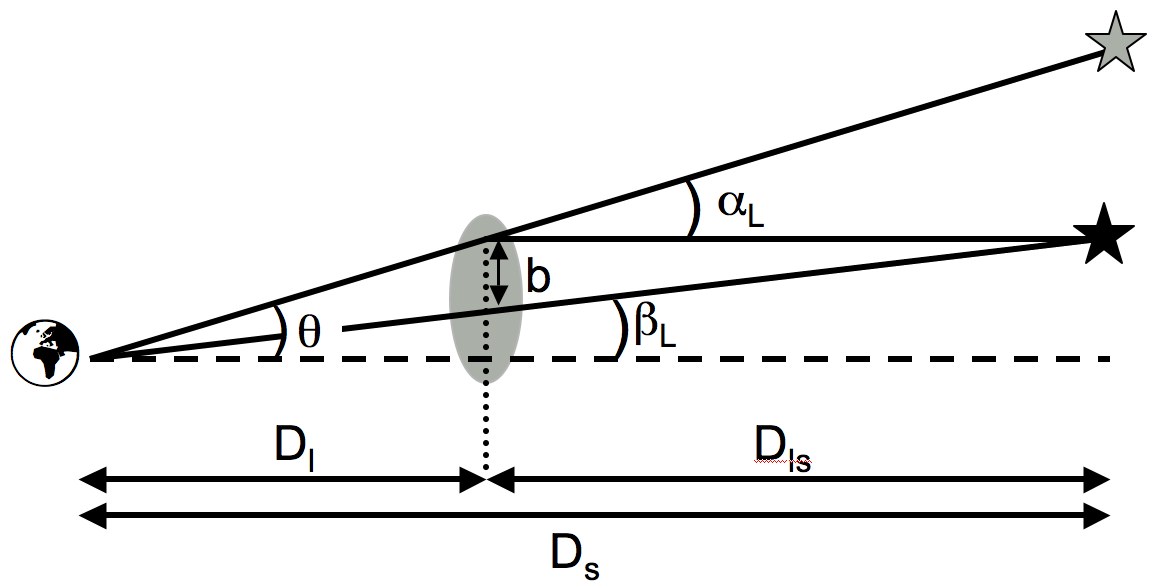
\includegraphics[scale=0.4]{plots_intro/LensDiagram.png}
\caption[Gravitational Lensing Diagram]{Diagram showing the geometry of gravitational lensing. Light from the background source is bent by an angle $\hat{\alpha}_{\rm L}$ when it passes near the gravitational lens (gray oval) on its way to the earth. While the actual source (black star) is at an angle $\beta_{\rm L}$ relative to the horizontal, its image (gray star) appears to be at an angle $\theta$. The angular diameter distances to the lens ($D_{\rm l}$), to the source ($D_{\rm s}$) and between the lens and source ($D_{\rm ls}$) are labeled.}
\label{plot:lensing}
\end{center}
\end{figure}

The fact that gravitational lensing directly probes the underlying density field along the line of sight is what makes the technique extremely valuable. All other methods for probing the matter distribution of the universe do not probe the mass itself (which is mostly dark matter), but rather the baryonic component of the mass -- stars, and interstellar gas and dust. While we expect the baryons to trace the underlying density of dark matter, there are many complicating factors (see \autoref{sec:Clusters}) that render the analogy lacking. Additionally, other means of measuring masses (such as using radial velocities) rely on assumptions about the virial equilibrium of a system which may not be satisfied.

Gravitational lensing is broadly divided into several branches depending upon the strength of the lensing effect. Strong lensing refers to the rarest and most obvious distortions, leading to images of giant arcs, Einstein rings, and multiple images of the same source. Strong lensing features are generally apparent to the eye (see \autoref{plot:abellcluster} for an example), whereas weak lensing and microlensing are not. The first observation of gravitational lensing producing multiple images was made by \citet{Walsh79} using a lensed quasar. The first gravitationally lensed arcs were discovered nearly a decade later by \citet{Lynds86} and \citet{Soucail87,Soucail88}. Currently, over one hundred strong gravitational lenses are known \citep{Browne03,Bolton08}. Strong lensing is very useful for accurately probing the dark matter halo mass profiles of galaxies and clusters of galaxies, often yielding detailed information on lens concentration \citep{Auger10} and substructure \citep{Mao98,Dalal02}. 

\begin{figure}
\begin{center}
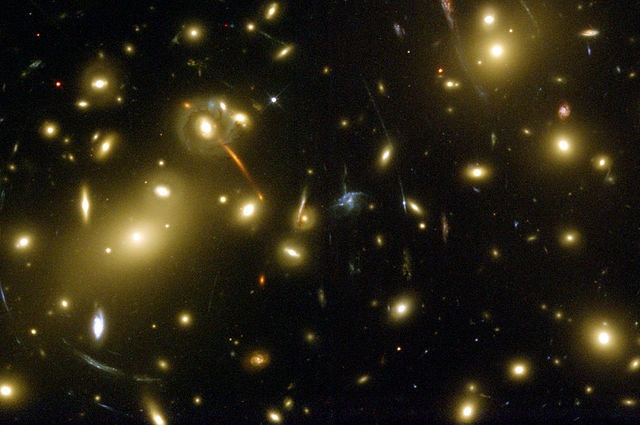
\includegraphics[scale=1.5]{plots_intro/Abell2218_Med.jpg}
\caption[Strong Lensing Image]{Abell 2218, a galaxy cluster at $z \sim 0.18$, yields a magnificent example of strong gravitational lensing. Many large arcs, which are highly distorted images of background galaxies, are easily visible in this image [Source: NASA].}
\label{plot:abellcluster}
\end{center}
\end{figure}

Weak lensing, just as the name implies, leads to much less significant distortions. The hallmark of weak lensing is that it is a statistical effect, only measurable using ensembles of many background sources and foreground lenses. Unlike the rarity of a strong lensing event, however, weak lensing is everywhere. Essentially all light rays are distorted at least a bit while traveling to us through the inhomogeneous gravitational fields of the universe. Weak lensing itself, and different approaches to measuring it, will be discussed in much more detail in \autoref{sec:Shear} and \autoref{sec:Mag} below. 

Finally, microlensing is the even weaker signature of gravitational lensing, wherein stars are lensed by low mass compact objects like black holes, brown dwarfs, and planets. Probably the most important use of microlensing has been the search for a significant \acf{MACHO} population in the Milky Way. \ac{MACHO}s were once considered a serious dark matter candidate until various microlensing experiments demonstrated that the mass density of \ac{MACHO}s was strongly insufficient to explain the missing mass in our galaxy \citep{Paczynski96,Wyrzykowski11,Sumi13}.

%%%%

\subsection{Weak Lensing Shear}
\label{sec:Shear}

Weak lensing shear is the component of weak lensing that deals with shape distortion of galaxy images. If all galaxies were intrinsically circular, or of known shape, then each individual background source would provide information on the gravitational field through which its light had propagated. Instead, however, galaxies take on a variety of shapes and orientations, and their unlensed representations are impossible to know. In order to proceed, weak lensing astronomers make two critical assumptions: (1) galaxy shapes can be approximated as elliptical, and (2) the orientation of these ellipses are random in the absence of gravitational lensing \citep{BS01}. The second point follows from the isotropy of the universe. Though only a few percent effect, characterization of any intrinsic alignments is an active area of research \citep[see e.g.][]{Hirata04,Heymans13}.

As illustrated in \autoref{plot:lensing}, the lens equation is given by 
\begin{equation}
\bm{\beta}_{\rm L} = \bm{\theta} - \bm{\alpha}_{\rm L},
\end{equation}
where we now use bold face to indicate angular positions with two components on the sky. The reduced deflection angle $\bm{\alpha}_{\rm L}$ is related to the deflection angle of \autoref{eqn:deflection} by $\bm{\alpha}_{\rm L} = (D_{\rm ls}/D_{\rm s})\bm{\hat{\alpha}}_{\rm L}$. The reduced deflection angle $\bm{\alpha}_{\rm L}$ can be expressed as the gradient of the lensing (or deflection) potential $\bm{\alpha}_{\rm L} = \nabla \psi$. The lensing potential $\psi(\bm{\theta})$ is the two-dimensional analogue to the Newtonian gravitational potential $\Phi$, and is given by \citep{NarayanBartelmann96}:
\begin{equation}
\psi(\bm{\theta}) = \frac{2}{c^2}\frac{D_{\rm ls}}{D_{\rm l} D_{\rm s}} \int \Phi(D_{\rm l} \bm{\theta},z){\rm d}z = \frac{1}{\pi} \int_{\mathbb{R}^2} \kappa(\bm{\theta'}) {\rm ln}|\bm{\theta} - \bm{\theta}'| {\rm d}^2 \theta'.
\end{equation}
Here $\kappa$ is known as the convergence, which encapsulates the magnification information to be described in \autoref{sec:Mag} below. Explicitly, the convergence is given by
\begin{equation}
\label{eqn:kappapartials}
\kappa(\bm{\theta}) =\frac{1}{2} \left( \frac{\partial^2 \psi(\bm{\theta})}{\partial\theta_1^2} + \frac{\partial^2 \psi(\bm{\theta})}{\partial\theta_2^2} \right),
\end{equation}
and another useful expression is the ratio
\begin{equation}
\label{eqn:kappa}
\kappa(\bm{\theta}) = \frac{\Sigma(\bm{\theta})}{\Sigma_{\rm crit}}.
\end{equation}
Here $\Sigma(\bm{\theta})$ is the two-dimensional surface mass density (with units of mass per area on the sky), and $\Sigma_{\mathrm{crit}}$ is the critical surface mass density of the lens \citep{Wright00}. The latter demarcates the separation between strong and weak gravitational lenses, depending critically on the geometry of the angular diameter distances between objects, given by
\begin{equation}
\label{eqn:sigcrit}
\Sigma_{\mathrm{crit}} = \frac{c^2}{4 \pi G} \frac{D_{\rm s}}{D_{\rm l} D_{\rm ls}}.
\end{equation}
Strong lenses (i.e. capable of forming multiple images) must have $\Sigma \ge \Sigma_{\mathrm{crit}}$ \citep{Schneider06_IntroGravLensCosmology}.

\begin{figure}
\begin{center}
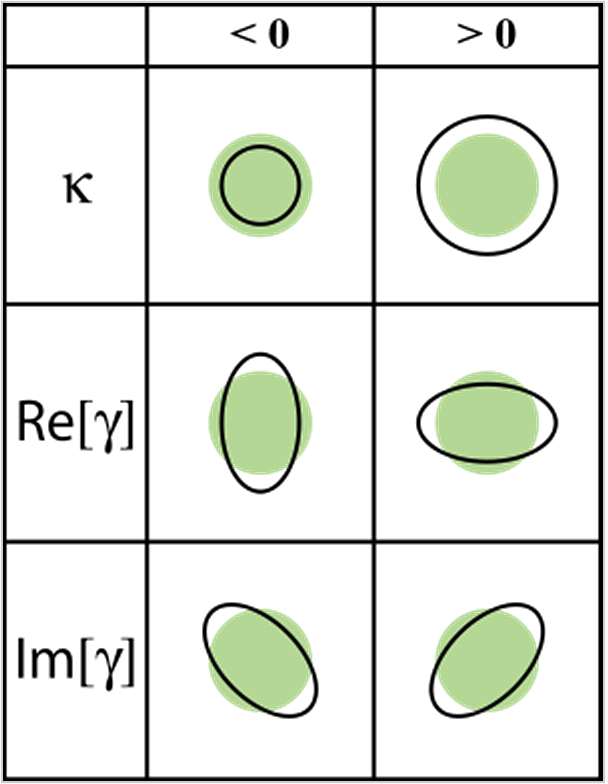
\includegraphics[scale=0.3]{plots_intro/kappa_gamma.png}
\caption[$\kappa$ and $\gamma$ Diagram]{Demonstration of the effect of convergence $\kappa$ and shear $\gamma$ on a circular source. Diagram shows the unlensed source (green circle) and the final lensed image (black outline) for positive and negative values of both $\kappa$ and the real and imaginary components of $\gamma$. [Source: TallJimbo/Wikimedia Commons/CC-BY-SA-3.0].}
\label{plot:kappagamma}
\end{center}
\end{figure}

The transformation of background objects from source (unlensed) to image (lensed) is described by the Jacobian (or amplification) matrix $\cal{A}$ \citep{DodelsonText}: 
\begin{equation}
\label{eqn:A}
{\cal A}(\bm{\theta}) = \frac{\partial \bm{\beta_{\rm L}}}{\partial \bm{\theta}}  = \left( \delta_{ij} - \frac{\partial^2 \psi(\bm{\theta})}{\partial \theta_{i} \partial \theta_j} \right) = \left( \begin{array}{cc}
{1-\kappa-\gamma_1} & {-\gamma_2} \\
{-\gamma_2} & {1-\kappa+\gamma_1} \\
\end{array} \right). 
\end{equation}
The two components of the shear $\gamma (\bm{\theta})$ can be expressed as derivates of the lensing potential:
\begin{equation}
\gamma_1 = \frac{1}{2} \left( \frac{\partial^2 \psi(\bm{\theta})}{\partial\theta_1^2} - \frac{\partial^2 \psi(\bm{\theta})}{\partial\theta_2^2} \right), 
\end{equation}
\begin{equation}
\gamma_2 = \frac{\partial^2 \psi(\bm{\theta})}{\partial\theta_1 \partial\theta_2}.
\end{equation}
The shear is often written as a complex number, $\gamma \equiv \gamma_1 + i\gamma_2 = |\gamma|{\rm e}^{2i\varphi}$. Here $|\gamma|$ and $\varphi$ indicate the amplitude and direction of distortion, respectively, which is unchanged when rotated by 180$^\circ$. An illustration of the meaning of each component of $\gamma$, as well as $\kappa$ is given in \autoref{plot:kappagamma}

We do not observe the true shear, but rather the reduced shear  $g(\bm{\theta}) = \gamma (\bm{\theta}) \left[1-\kappa (\bm{\theta}) \right]^{-1}$. We can thus rewrite the Jacobian matrix as:
\begin{equation}
\label{eqn:Ag}
{\cal A}(\bm{\theta}) = (1-\kappa) \left( \begin{array}{cc}
{1-g_1} & {-g_2} \\
{-g_2} & {1+g_1} \\
\end{array} \right). 
\end{equation}
In the regime of weak lensing, the convergence and shear are small, $\kappa \ll 1$ and $| \gamma| \ll 1$. Therefore it is often safe to assume that $\gamma \approx g$ \citep{Schneider06_WeakGravLens}.

The observed brightness distribution of a galaxy image $I(\bm{\theta})$ is not in general perfectly elliptical, but we can approximate it as an ellipse in the following manner. The center of the brightness distribution of the image is
\begin{equation}
\bm{\bar{\theta}} \equiv \frac{\int {\rm d}^2\theta I(\bm{\theta}) q_I( I(\bm{\theta})) \bm{\theta}}{\int {\rm d}^2\theta I(\bm{\theta}) q_I( I(\bm{\theta}))},
\end{equation}
where $q_I( I(\bm{\theta}))$ is some weight function, and we assume that the galaxy image of interest is isolated on the sky. To describe ellipticity we will be interested in the second brightness moments of the source, contained in the tensor
\begin{equation}
Q_{ij} = \frac{\int {\rm d}^2\theta I(\bm{\theta}) q_I( I(\bm{\theta})) (\theta_i - \bar{\theta_i})(\theta_j - \bar{\theta_j})}{\int {\rm d}^2\theta I(\bm{\theta}) q_I( I(\bm{\theta}))},
\end{equation}
where $i,j \in (1,2)$ \citep{Schneider06_WeakGravLens}. The size $\omega$ of the galaxy image is just a function of the diagonal components of this matrix,
\begin{equation} 
\label{eqn:size}
\omega = (Q_{11}Q_{22} - Q_{12}^2)^{1/2},
\end{equation}
while the shape, or ellipticity, of the image involves the off-diagonal elements:
\begin{equation} 
\chi \equiv \frac{Q_{11} - Q_{22} + 2i Q_{12}}{Q_{11} + Q_{22}} ,
\end{equation}
\begin{equation} 
\epsilon \equiv \frac{Q_{11} - Q_{22} + 2i Q_{12}}{Q_{11} + Q_{22} + 2(Q_{11}Q_{22} - Q_{12}^2)^{1/2}}.
\end{equation}
The complex ellipticity can be characterized by either of $\chi$ or $\epsilon$, which are simply related and interchangeable (in different situations one may be easier to work with) \citep{BS01}. 

In analogy with the image center $\bm{\bar{\theta}}$ and tensor of second brightness moments $Q_{ij}$, one can define the same quantities for the unlensed source center $\bm{\bar{\beta}}$ and tensor of second brightness moments $Q_{ij}^{(s)}$. The relation between the source and image tensors is
\begin{equation}
Q^{(s)} = {\cal A} Q {\cal A}^{\rm T} = {\cal A} Q {\cal A},
\end{equation}
where ${\cal A} \equiv {\cal A}(\bm{\theta})$ is the Jacobian defined in \autoref{eqn:A} and \autoref{eqn:Ag}. The observed source ellipticity $\epsilon$ is related both to the shear caused by weak lensing, and to the intrinsic ellipticity $\epsilon^{(s)}$ of the unlensed background source:
\begin{equation} 
\epsilon^{(s)} = 
    \begin{cases}
        \frac{\epsilon - g}{1-g^*\epsilon}, & \text{for} |g| \le 1 \\
        \frac{1-g\epsilon^*}{\epsilon^* - g^*}, & \text{for} |g| > 1.
    \end{cases}
\end{equation}
If we average over many background sources that are randomly oriented, then the average intrinsic ellipticity $\langle \epsilon^{(s)} \rangle = 0$ and we can apply the weak lensing approximation to conclude that $\gamma \approx g \approx \langle \epsilon \rangle \approx  \langle \chi \rangle /2$ \citep{BS01}. 

In this thesis we are concerned with a particular manifestation of gravitational lensing -- lensing by galaxy clusters. If we consider an circularly symmetric mass density on the sky (an idealized galaxy cluster), then we expect the shear distortion to be oriented tangential to the center of the lens. It is therefore useful in cluster lensing (and also in galaxy-galaxy lensing) to express the shear in terms of tangential and rotated (or cross) components:
\begin{equation}
\gamma_{\rm t} = -{\rm Re}\left[ \gamma {\rm e}^{-2i\phi} \right],  
\end{equation}
\begin{equation}
\gamma_{\rm r} = -{\rm Im}\left[ \gamma {\rm e}^{-2i\phi} \right].
\end{equation}
Here the angle $\phi$ is the azimuthal angle measured about the center of the lens \citep{Schneider06_WeakGravLens}. The rotated shear (which would represent a curl component) should be consistent with zero, and is often used as a check of systematic effects. Even though any single galaxy cluster (or other lens) is likely not perfectly azimuthally symmetric, we expect a stack of many galaxy clusters to yield a symmetric profile on average.

\begin{figure}
\begin{center}
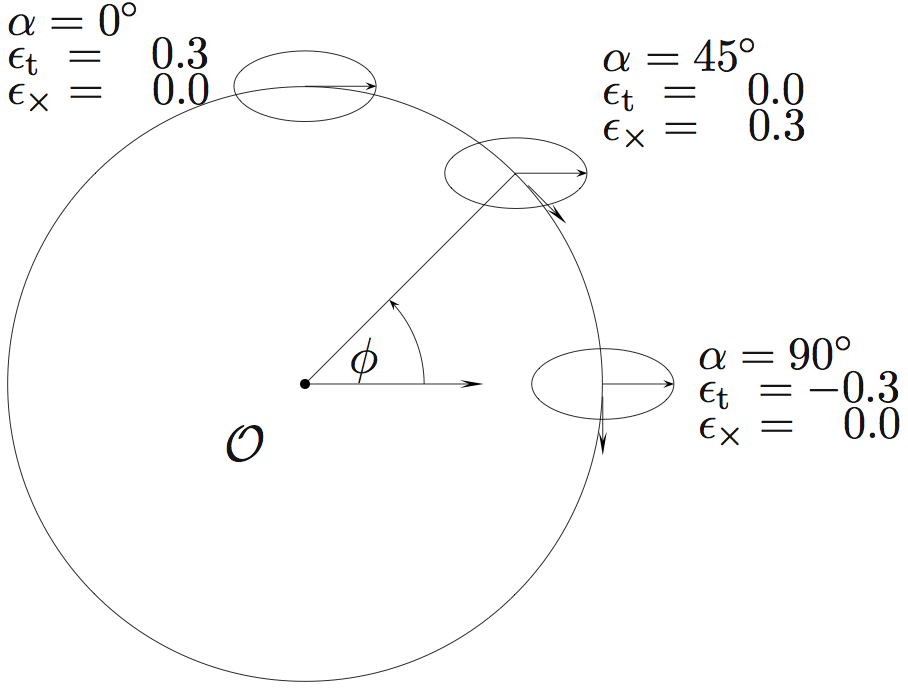
\includegraphics[scale=0.3]{plots_intro/ShearComponents.png}
\caption[Tangential Shear]{Diagram illustrating the components of ellipticity, when decomposed into a tangential and cross component relative to the center of a gravitational lens. As described in the text of \autoref{sec:Shear}, the ellipticities $(\epsilon_{\rm t},\epsilon_{\times})$ are equivalent to the shear $(\gamma_{\rm t},\gamma_{\rm r})$ if they have been averaged over many sources that were randomly oriented in the absence of lensing. The angle $\phi$ measures the azimuthal position of the source about the center of the gravitational lens. [Source: \citet{Schneider06_WeakGravLens}].}
\label{plot:shearcomponents}
\end{center}
\end{figure}

Similar to the surface mass density representation of the convergence (\autoref{eqn:kappa}), we can then relate the tangential shear to the differential surface mass density of the lens:
\begin{equation}
\gamma_{\rm t}(\theta) = \frac{\Delta\Sigma(\theta)}{\Sigma_{\rm crit}},
\end{equation}
where $\theta$ now specifies the radial angle of separation between the lens center and the source image. The differential surface mass density is defined to equal the difference between the average surface mass density interior to $\theta$ and the surface mass density at $\theta$ \citep{Wright00}: 
\begin{equation}
\Delta\Sigma(\theta) \equiv \overline{\Sigma}(< \theta) - \Sigma(\theta).
\end{equation}
Given an expression for the mass density profile of a gravitational lens, and angular diameter distances involved, the expected tangential shear profile can be calculated. Useful models for galaxy cluster masses, and the resulting $\gamma_{\rm t}(\theta)$ and $\Delta\Sigma(\theta)$ profiles, will be given in \autoref{sec:Clusters}.

%%%%

\subsection{Weak Lensing Magnification}
\label{sec:Mag}

Gravitational lensing causes the magnification of background galaxies due to the isotropic focusing of the lensed light rays (whereas shear arises from the anisotropic component). Magnification $\mu(\bm{\theta})$ is related to the determinant of the Jacobian, 
\begin{equation}
\mu  = \frac{1}{{\rm det}{\cal A}} = \frac{1}{(1-\kappa)^2 - |\gamma|^2}.
\end{equation}
In the weak lensing limit ($|\gamma| \ll 1$), the magnification is simply a measure of the convergence of a lensing mass, $\mu \approx 1+2\kappa$, where $\kappa$ is defined in \autoref{eqn:kappapartials} and \autoref{eqn:kappa} \citep{Schneider06_IntroGravLensCosmology}. For the case of circularly symmetric sources we can write $\mu = (\theta/\beta_{\rm L})({\rm d}\theta/{\rm d}\beta_{\rm L})$
\citep{NarayanBartelmann96}. Conceptually, magnification can be understood as the stretching of solid angle on the sky, which causes the amplification of source flux, since lensing conserves surface brightness. This directly leads to a change in source size $\omega = \mu(\bm{\theta}) \omega^{(s)}$, where size is defined in \autoref{eqn:size} \citep{BS01}.

In general, two different approaches can be taken to measure magnification: (1) quantifying sizes of galaxies behind lenses and measuring lensing-induced changes, or (2) detecting the effect on background source number density that ensues as a result of amplification in a flux-limited survey. This thesis focuses on the latter approach. The former method suffers from many of the limitations facing shear analysis, and will be discussed briefly in \autoref{sec:VS} below. 

\begin{figure}
\begin{center}
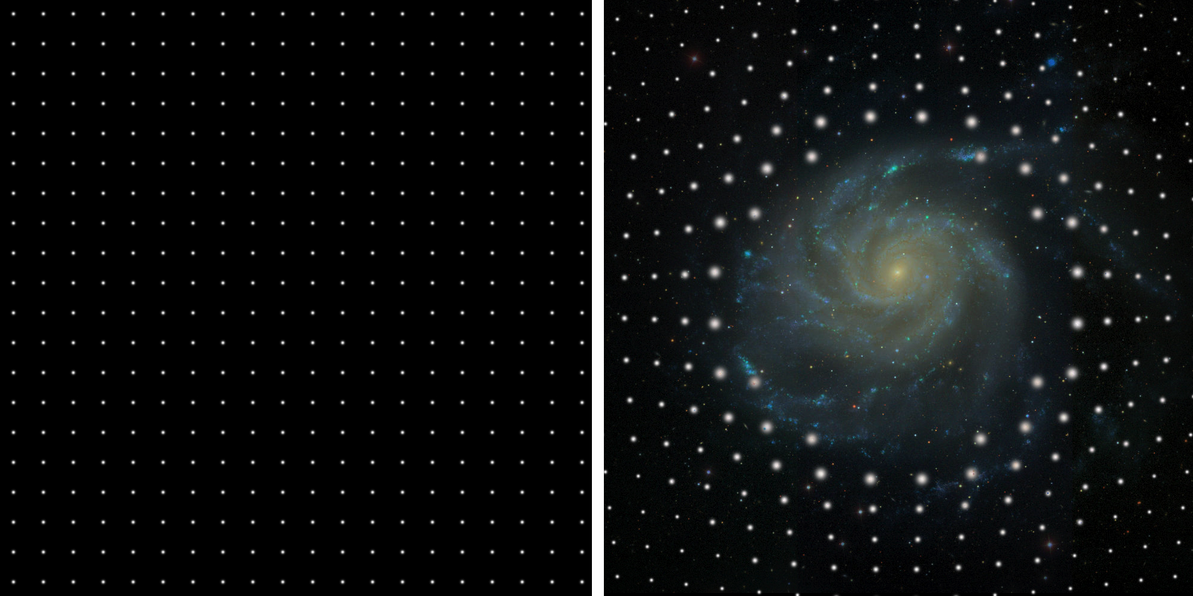
\includegraphics[scale=0.4]{plots_intro/Magnification.png}
\caption[Magnification Illustration]{Highly exaggerated illustration of the two effects of magnification (dilution and amplification) by a massive foreground galaxy. The left panel shows an idealized set of unlensed sources, the right panel shows the effect of gravitational lensing. Dilution refers to the stretching of solid angle on the sky, which reduces background source number density. Since lensing conserves surface brightness, a consequence is that source flux is amplified. [Source: Joerg Colberg, Ryan Scranton, Robert Lupton, \ac{SDSS}].}
\label{plot:magnification}
\end{center}
\end{figure}

Define $n_0(f,z){\rm d}f{\rm d}z$ to be the intrinsic (unlensed) number of galaxies per solid angle within ${\rm d}f$ of flux $f$ and ${\rm d}z$ of redshift $z$. The cumulative lensed number density detectable (i.e. brighter than $f$) in an astronomical survey will then be:
\begin{equation}
n(>f,\bm{\theta},z) = \frac{1}{\mu(\bm{\theta},z)} n_0\left(\frac{>f}{\mu(\bm{\theta},z)},z\right).
\end{equation}
In this equation we can see that magnification affects the source number densities in two ways. The prefactor $1/\mu$ represents the stretching of apparent solid angle, and decreases the number density on the sky. Meanwhile, the denominator in the argument of $n_0$ implies that sources will be detectable to a fainter intrinsic magnitude, effectively increasing the observed source number density if there exist sources fainter than the detection limit of the survey \citep{Schneider06_WeakGravLens}. An illustration of the two effects of magnification is given in \autoref{plot:magnification}.

Since magnification affects the background source number densities in these two opposing ways, we require knowledge of the intrinsic source number densities as a function of brightness, in order to predict or interpret our magnification observations. Typically, astronomical sources such as galaxies contain relatively few very bright members and are much more numerous towards the faint end. If we approximate the slope of the number density in a narrow flux bin as a power law $n_0(f) \propto f^{-\alpha}$, then we have
\begin{equation}
\frac{n(>f)}{n_0(>f)} = \mu^{\alpha-1}.
\end{equation}

Unfortunately, instead of using flux, astronomers frequently characterize source brightness using the ancient-Greek-inspired system of magnitudes. The apparent (observed) magnitude of an object with flux $f$ is
\begin{equation}
m \equiv -2.5 {\rm log}_{10}(f/f_{\rm x}),
\end{equation}
where $f_{\rm x} = 2.53 \times 10^{-8} \ {\rm W}/{\rm m}^2$ is a reference flux. Bright sources have smaller apparent magnitudes. Absolute magnitude $M$ can be defined similarly, but relative to a reference luminosity. Its relation to apparent magnitude can be expressed as $M=m-5{\rm log}_{10}(d_L/10{\rm pc})$, where $d_L$ is the luminosity distance in \autoref{eqn:dL} \citep{RydenText}. In terms of apparent magnitudes we can relate the lensed and intrinsic number densities using the equation
\begin{equation}
\label{eqn:nofm}
n(m,z){\rm d}m = \mu^{\alpha -1} n_0(m,z){\rm d}m,
\end{equation}
where we now define $\alpha$ explicitly according to
\begin{equation}
\alpha \equiv \alpha(m,z) = 2.5 \frac{\mathrm d}{\mathrm d \it m} \log n_0(m,z).
\label{alpha}
\end{equation}
The form of \autoref{eqn:nofm} was first demonstrated by \citet{Narayan89}, who applied it to lensed quasar number densities, but it can be generalized to any galaxy type as long as one has a means of obtaining the slope of the number counts $\alpha$.

Returning to the question of whether gravitational lensing magnification will cause an increase or decrease in observed number densities of background sources, we find that the answer depends precisely on the value of $\alpha$. Sources for which $\alpha -1 > 0$ will appear to be correlated on the sky with a lens position, while sources with $\alpha -1 < 0$ will be anti-correlated, as a dearth of objects will be observed in the vicinity of a lens.  The number density of galaxies for which the intrinsic number count slope gives $\alpha -1 \approx 0$ will essentially be unaffected by lensing magnification, as the dilution and amplification effects will cancel, and no correlation signal will be observed for these objects \citep{Scranton05}. The brightest sources, which usually have steep number counts, will exhibit an {\it increase} in number density when lensed, as the amplification allows more objects to be detected, while the number density of the faintest sources, having relatively shallow number counts, will {\it decrease} \citep{Narayan89}.

Lensing magnification has had an interesting history. During the 1970s and '80s several studies showed that bright quasars were correlated on the sky with foreground galaxies \citep{SeldnerPeebles79,Arp81,Webster88,Narayan89}. The reason for this association was hotly debated, with some astronomers even arguing for physical associations of the objects \citep{Arp87}. The proponents of the lensing interpretation were frequently obtaining results discrepant with eachothers' as well as with the expected lensing signal strength \citep[see e.g.][]{Schneider92} through the end of the 20$^{\rm th}$ century. The first convincing magnification detection was made by \citet{Scranton05}, using 200,000 quasars lensed by 13 million galaxies in the \acf{SDSS}.

Quasars are appealing background sources for magnification studies for two reasons. First of all, their high redshifts ensure that they are well separated from the foreground lenses, which is important so that physical associations due to gravitational attraction do not contaminate the lensing signal. Secondly, their steep number counts yield high values for the slope $\alpha(m,z)$ which leads to strong positive correlations with the lenses. More recently, \acf{LBG} sources have also been used successfully in magnification studies by \citet{Hildebrandt09b},\citet{Morrison12}, and \citet{Hildebrandt13} and by the author of this thesis in \citet{Ford12} and \citet{Ford14} (see \autoref{ch2}and \autoref{ch3}). These galaxies tend to also have high $\alpha(m,z)$ values, but more care must be taken to ensure redshift separation from the lenses involved.

\subsection{Magnification vs. Shear}
\label{sec:VS}

The shear approach to weak lensing has dominated the field for the last several decades. Early work by \citet{Schneider00} showed that shape information had less intrinsic scatter than sizes or number counts, and concluded that very little was gained by including magnification along with shear. A review article by \citet{BS01} compared the signal-to-noise ratios of shear and magnification, finding the shear signal-to-noise to be at least 5 times larger than for magnification. This comparison included several simplifying assumptions, like equal number densities of sources for shear and magnification, and a number count slope of $\alpha=0.5$. However, \ac{LBG}s and quasars can have $\alpha$ values of several, at the bright end of the luminosity function, and magnification with number counts can certainly include many times the number of sources relevant for a shear analysis.

One of the really attractive aspects of magnification is its ability to be applied in regimes where the shear technique starts to fail. Since shear studies require accurate measurements of galaxy shapes, in order for a source to be used at all, it must necessarily be well resolved. Specifically, for lenses at high redshift, and for ground-based surveys facing the extra complication of blurring to to atmospheric seeing, the number density of background sources for which shear can be well-determined is greatly reduced \citep{Waerbeke10}.  This is in stark contrast to magnification studies using source number densities, which have no such requirement for the sources to be resolved at all.  In principle only source magnitudes, redshifts, and positions relative to a lens must be known.  This simple fact makes it possible to extend weak lensing magnification analyses to a much higher redshift than possible for shear, and allows a much higher source density to be included in the analysis \citep{LHJM10}.  

Shear is susceptible to an issue known as the mass sheet degeneracy. This is the fact that, since shear probes differential mass profiles, $\Delta\Sigma(\theta)$, adding a constant mass sheet across an entire lens does not change the measured shear \citep{Falco85,SchneiderSeitz95}. Any weak lensing shear measurement is thus left with some ambiguity (although in practice, if the survey area is large enough, this is usually not a concern). Magnification, which directly probes the surface mass density, $\Sigma(\theta)$, can be used to break this mass sheet degeneracy \citep{Broadhurst95}. The combination of shear and magnification, in order to circumvent this degeneracy has been demonstrated in a series of cluster analyses by \citet{Umetsu11,Umetsu13,Umetsu14}.

Some progress has been made in terms of measuring magnification using source size information \citep{Huff14,Schmidt12}. Unfortunately, the approach of measuring size magnification suffers from many of same limitations as the shear technique, since it also requires quantifying the spatial extent of sources which must necessarily be well resolved. Although back-of-the-envelope calculations by \citet{BS01} showed a larger signal-to-noise ratio for size than for number density magnification, \citet{Schneider06_WeakGravLens} explains how the Point Spread Function circularizes the sources, and that seeing-convolved image sizes are even more difficult to measure than shapes. A related alternative approach to measuring magnification by using the modified redshift distributions of lensed background sources was originally proposed by \citet{Broadhurst95}, and recently demonstrated on observational data by \citet{Coupon13}.

Because the constraint on source resolution is considerably relaxed, ground-based observations can be incorporated to a greater degree with magnification (using number counts) than for shear (or size magnification), as we are not concerned with correcting for the smearing of the image due to the atmospheric Point Spread Function. From the financial perspective, these types of magnification studies are therefore extremely cheap to carry out, since the excellent resolution of space-based telescopes is not required \citep{Hildebrandt09b}. 

The bottom line regarding magnification is that it provides gravitational lensing information that is independent of, and complementary to, the information obtained from a weak lensing shear analysis. Since magnification with source number densities (which is the approach taken in \autoref{ch2} and \autoref{ch3} of this thesis) essentially imposes no additional constraints on a weak lensing shear survey, the ability to perform a magnification analysis comes along for free. Any costless source of cosmological information ought to be investigated and exploited in full. See \citet{Waerbeke10}, \citet{RozoSchmidt10}, and \citet{Umetsu11}, for more detailed discussions of the benefits of combining magnification with shear in gravitational lensing studies.


%%%%%%%%%%%%%%%%%%%%%%%%%%%%%%%%%%%%%%%%%%%%%%%%%%%%%%%%%%%%%%%%%%%%%
\section{Galaxy Clusters}
\label{sec:Clusters}

Clusters of galaxies represent the largest and most massive gravitationally-bound systems to have formed thus far in our universe. They range from associations of only a few nearby galaxies, called groups, all the way up to very rich clusters containing many thousands of members. The distinction between groups and clusters is not well defined, and this thesis will largely use the word ``clusters'' as a blanket term covering all groupings of galaxies. Clusters themselves are observed to clump together into enormous superclusters.

Galaxies were first recognized to cluster together by Charles Messier in 1784, and then independently by F. Wilhelm Herschel in the early 19$^{\rm th}$ century, long before they were actually recognized as very distant galaxies similar to our own (they were called ``nebulae'') \citep{Biviano00}. The first cluster masses were estimated by \citet{Zwicky33}, but it wasn't until the first comprehensive catalog of over two thousand clusters was produced by \citet{Abell58} that the study of galaxy clusters really began to take off. Today hundreds of thousands of galaxy clusters have been cataloged and studied \citep[see e.g.][]{Wen12}.

Because they harbor the deepest gravitational potentials in the universe, clusters are unique laboratories for studying the highest energy phenomena since the big bang. They can be used a testing grounds for general relativity, and gravitational structure formation. Baryonic processes of the intergalactic medium, high energy plasma physics, and the interplay with member galaxies and galaxy evolution, can all be explored using galaxy clusters \citep{Kravtsov12}. This section will discuss the two key uses for studying galaxy clusters -- to constrain cosmology (\autoref{sec:ClusterCosmo}) and to understand astrophysical processes (\autoref{sec:ClusterAstro}) -- with an attempt to highlight the significant aspects of these areas that are relevant to this thesis.

\subsection{Clusters for Cosmology}
\label{sec:ClusterCosmo}
Clusters of galaxies represent the high-mass end of structure formation in the universe, and the most recent objects to have collapsed gravitationally. Quantifying cluster number density as a function of mass can be a sensitive probe of cosmology. Two cosmological parameters that are of particular importance for the study of galaxy clusters are $\Omega_{\rm m}$ and $\sigma_8$. The first, already discussed in \autoref{sec:Cosmology}, is the matter content of the universe expressed as a fraction of the total energy density. The second parameter, $\sigma_8$, is known as the normalization of the matter power spectrum. It can also be described as the variance in the mass contained within spheres randomly located throughout the universe, with comoving radius $8 h^{-1}$Mpc (hence the subscript ``8'') \citep{Voit05}.

The fact that our universe even contains galaxies and other structures, means that the universe is not perfectly homogeneous. The canonical description is that, at early times there existed slight perturbations in the density field, which underwent gravitational collapse to eventually form the varied structures we observe today. If the average density was $\langle \rho_m \rangle$, then these density perturbations as a function of position can be written as
\begin{equation}
\delta(x) = \frac{\rho_m(x) - \langle \rho_m \rangle}{\langle \rho_m \rangle}.
\end{equation}
The Fourier components of the density perturbations are $\delta_{\rm k}(k) = \int \delta(x) {\rm e}^{i {\bm k} \cdot {\bm x}}{\rm d}^3x$. 

If we believe that the universe is indeed isotropic, and that these perturbations $\delta(x)$ can be described as a Gaussian random field (the simplest case scenario), then we can fully characterize them using the isotropic power spectrum $P(k) \equiv \langle | \delta_{\rm k} |^2 \rangle$ \citep{Kravtsov12}. The power spectrum is often approximated as a power law $P(k) \propto k^n$, where $n=1$ is the special scale-invariant case proposed around the same time by \citet{Harrison70,PeeblesYu70,Zeldovich72}. Recent measurements by \citet{PlanckXVI} have shown that $n \approx 0.96$.

Defining a spherical window function $W(r)$, and its Fourier transform $W_k$, we can write the variance on mass scale ${\cal M}$ as 
\begin{equation}
\sigma^2 \equiv \left\langle \left| \frac{\delta {\cal M}}{\cal M} \right|^2 \right\rangle = \frac{1}{(2\pi)^3} \int P(k) |W_k|^2 {\rm d}^3k.
\end{equation}
Thus $\sigma_8$ is simply a special case of the square root of the above expression, wherein a top hat window function of radius $8 h^{-1}$Mpc is used.\footnote{The top hat window function is constant inside the $8 h^{-1}$Mpc radius, zero outside of it, and is normalized so it integrates to one.} This particular radius is historical in nature, simply chosen because $(\delta {\cal M}/{\cal M}) \sim 1$ in spheres of this volume, but it remains widely used in the cosmological literature today \citep{Voit05}. Better constraints now give $\sigma_8 \approx 0.83$ \citep{PlanckXVI}.

At first, when the density constrast was small $\delta(x) \ll 1$, the perturbations simply expanded along with the universe. The modes grew independently, according to the linear growth function \citep{Voit05}:
\begin{equation}
D(a) \propto \frac{\delta \rho}{\rho} \propto \frac{\dot{a}}{a} \int_0^a \frac{{\rm d}a}{\dot{a}^3}.
\end{equation}
Later, as they entered each other's horizon, the overdense regions grew by attracting surrounding matter. Once they reach a critical density contrast $\delta_c$, they collapsed gravitationally and decoupled from the global expansion \citep{Schneider06_IntroGravLensCosmology}. Smaller overdensities merged together to form larger structures, in what is known as hierarchical structure formation. A full mathematical description of the growth of structure is beyond the scope of this introduction,  and the reader is referred to important early papers \citep[e.g.][]{PS74,GottRees75} or more recent excellent reviews on the subject \citep[e.g.][]{Voit05,Schneider06_IntroGravLensCosmology,Kravtsov12}. 

A common approach to extracting cosmological information from galaxy clusters involves measuring the cumulative number density (comoving) of clusters above some mass threshold.  This important quantity $n_M (M,z)$ is known as the cluster mass function. In the original formalism of \citet{PS74} the cluster mass function is given by
\begin{equation}
n_M (M,z) = \frac{\Omega_{\rm m} \rho_{\rm crit}(z=0)}{M} {\rm erfc}\left[ \frac{\delta_c}{\sqrt{2}\sigma(M,z)} \right].
\end{equation}
Improvements have been made on the Press-Schechter formalism, most notably by \citet{Sheth99} and \citet{Jenkins01}, generalizing to ellipsoidal perturbations and improving parameterizations based on cluster simulations. The cluster mass function $n_M$ depends very specifically on the meaning of the mass of a cluster. A common choice, which will be used throughout this thesis, is the mass parameter $M_{200}$. This is the total mass interior to a radius $R_{200}$, within which the average density is 200 times the critical energy density of the universe, $\langle \rho (r<R_{200}) \rangle = 200 \rho_{\rm crit}(z)$.

There are several difficulties in connecting galaxy cluster observations to theories of structure formation in cosmology. Clusters evolve over time, but we cannot observe the collapse of an individual halo because of the time scales involved. Instead we must make inferences by observing ensembles of clusters at different redshifts. Other issues are the observational difficulties associated with compiling pure and complete samples of galaxy clusters, using techniques that nearly always probe some visible tracer of the cluster dark matter halo. Finally, it is very difficult to accurately know the true mass $M$ that appears in the cluster mass function. Gravitational lensing is the most promising method for obtaining accurate cluster masses, and the work in this thesis is aimed at improving these estimates further, especially for higher redshift clusters. Future experiments may build upon this work to use galaxy clusters to improve constraints on cosmology.

\textcolor{red}{Include power spectrum visualization (pg 81 Schneider hardcopy)?}

\subsection{Clusters for Astrophysics}
\label{sec:ClusterAstro}

Other stuff... \citep{Voit05} Be sure to include NFW profiles and $\Delta\Sigma$ profiles for clusters, as claimed at end of shear section.

\textcolor{red}{\begin{itemize}\item cluster intro pg 30+ Schneider ecopy \item NFW on pg 76, of Schneider hardcopy \item halo abundance, power spectrum, pg 67+/- Schneider hardcopy \item good power spectrum visualization pg 81 Schneider hardcopy \end{itemize}}


%%%%%%%%%%%%%%%%%%%%%%%%%%%%%%%%%%%%%%%%%%%%%%%%%%%%%%%%%%%%%%%%%%%%%%
\section{Impact of this Thesis}
\label{sec:Impact}

This work contained in this thesis has pushed the boundaries of what knowledge can be extracted from weak lensing surveys. By including intrinsically smaller and fainter background sources, which cannot be used in conventional weak lensing studies, we pave the way for a more optimal use of survey data. These gravitationally-lensed sources, which are too small for reliable shape or size measurements, can still be included in a lensing analysis by using the flux magnification formalism described in \autoref{sec:Mag}. The author of this thesis has proven the utility of measuring magnification, through several key publications which appear as chapters in this work, and carried out thorough studies of the systematic effects which provide limitations. 

Prior to this thesis research, weak lensing was dominated by the shear method. This was originally motivated by some early work showing that the signal-to-noise for shear was several times larger than for magnification \citep{Schneider00}. While it is true that, for a fixed sample of galaxies, there is less scatter in galaxy shapes than in galaxy positions, the latter is far easier to measure. This simple fact has motivated the research herein. As lensing studies push to higher redshift, and increasingly rely on blurry ground-based data, we have elevated confidence in our measurements of source positions over difficult shape determinations. 

When this thesis work began, only a handful of magnification studies had been completed. The first ground-breaking theoretical formulation of how number densities of sources could be used to measure masses of clusters was laid out in 1995 by \citet{Broadhurst95}, but it took another 20 years before the first convincing observational detection was made \citep{Scranton05}. Following this significant $8\sigma$ detection of galaxy-magnified quasars in the \ac{SDSS}, several studies followed, achieving magnification detections for lensing of normal galaxies \citep{Hildebrandt09b}, and of blue galaxies behind strong lensing clusters \citep{Umetsu11}. These studies all stopped short of deriving scientifically useful results from the magnification measurements -- they either represented proof-of-concept studies for a new technique, or they demonstrated consistency with a lensing interpretation of the signal.

The work in this thesis made major steps forward in the area of lensing magnification. The author performed the first-ever measurement of magnification by stacked galaxy groups in 2012 (See \autoref{ch2}). This particular work was also the first time that shear and magnification mass estimates and signal-to-noise had been compared \citep{Ford12}. Following this influential work in the \acf{COSMOS} survey, the thesis author transitioned focus to the much larger astronomical survey known as the \acf{CFHTLenS}. 

Two important studies resulted from magnification analyses of the \ac{CFHTLenS} for this thesis (See \autoref{ch3} and \autoref{ch4}). First of all, the most significant magnification detection thus far (at $9.7\sigma$) was published in \citet{Ford14}. More importantly, however, that work moved beyond simple magnification-detection to actual science. The thesis author measured masses of stacked galaxy clusters binned as a function of different attributes (redshift and richness), and the dependence of a magnification signal on these parameters was seen for the first time. A mass-richness scaling relation was determined solely from the magnification results, which is a useful tool for making cosmological inferences from optical cluster surveys, as discussed in \autoref{sec:Clusters}. 

This work contained the important inclusion of a means of accounting for one of the dominant systematic effects for magnification, the contamination of the background sources with low-redshift objects. The formalism was extended from earlier work by \citet{Hildebrandt13}, but allowing for different contamination fractions and models for the halo occupation distribution of the galaxy contaminants. This was the first time that galaxy cluster lenses could be used for magnification in a redshift range where there was known source contamination. Prior to this work, the redshift ranges of overlap had to be avoided because the physically-induced cross-correlations of lens and source objects overwhelmed, and could not be separated from, the magnification signal.

Arguably the most important magnification result in all the literature to date is contained in \autoref{ch4} of this thesis. After the semi-blind magnification analysis of \citet{Ford14}, \citet{Ford15} followed suit with an identical treatment of the same cluster sample, but this time using the weak lensing shear approach. This study contained a detailed comparison between cluster masses measured with the two independent techniques, as a function of different cluster attributes, and contained valuable insights regarding systematic effects that are still important to resolve for magnification. Moving forward, this work frames the case for including magnification, and also pin-points some important issues that must be addressed in future work (see \autoref{ch:conc}).

%%%%%%%%%%%%%%%%%%%%%%%%%%%%%%%%%%%%%%%%%%%%%%%%%%%%%%%%%%%%%%%%%%%%%%
\section{Thesis Overview}
\label{sec:Overview}

The body of this thesis is composed of three published studies that develop the weak gravitational lensing magnification technique, particularly for the study of galaxy clusters, and compare with results using the complementary and much more ubiquitous weak lensing shear approach:
\begin{itemize}
\item \autoref{ch2} contains the first magnification study of galaxy groups and first comparison with shear for stacked lens samples. The data are X-ray selected groups, and high-redshift \ac{LBG}s in the \ac{COSMOS} field.
\item \autoref{ch3} represents the highest-significance magnification detection, and the first magnification study that could be binned as a function of cluster parameters. The data are optically-selected galaxy clusters and high-redshift \ac{LBG}s in the \ac{CFHTLenS} field.
\item \autoref{ch4} is the follow-up shear analysis of the same cluster sample presented in the previous chapter, using the \ac{CFHTLenS} shear catalog for background source shape measurements.
\end{itemize}
Finally, \autoref{ch:conc} wraps up with conclusions on the topic of cluster studies using both magnification and shear, and briefly outlines future directions for progress within the field.

%%%%%%%%%%%%%%%%%%%%%%%%%%%%%%%%%%%%%%%%%%%%%%%%%%%%%%%%%%%%%%%%%%%%%%
\endinput
Any text after an \endinput is ignored.
You could put scraps here or things in progress.
